%&latex
\documentclass[a4paper]{report}
\usepackage{commons/commons}
\usepackage{commons/note_style}
\usepackage[normalem]{ulem}
\usepackage{comment}
\usepackage{titlesec}
\titleformat{\chapter}[display]
  {\normalfont\sffamily\big\bfseries\color{black}}
  {\chaptertitlename\ \thechapter}{5pt}{\huge}
%\excludecomment{figure}

\def\ojoin{\setbox0=\hbox{$\bowtie$}%
  \rule[-.02ex]{.25em}{.4pt}\llap{\rule[\ht0]{.25em}{.4pt}}}
\def\leftouterjoin{\mathbin{\ojoin\mkern-5.8mu\bowtie}}
\def\rightouterjoin{\mathbin{\bowtie\mkern-5.8mu\ojoin}}
\def\fullouterjoin{\mathbin{\ojoin\mkern-5.8mu\bowtie\mkern-5.8mu\ojoin}}
\usepackage{amsbsy}
\usepackage{amstext}


\begin{document}

%+Title
\title{Advanced Database Quicksheet}
\author{Daniel D. Zhang, \\ Based on \textit{Database Systems - The Complete Book}}
\date{Fall 2015. \today}
\maketitle
%-Title

%+Abstract
%\begin{abstract}
%This is the notes for CSE 232A.
%\end{abstract}
%-Abstract

%+Contents
\tableofcontents
%-Contents
\chapter*{Preface}
\section*{Preclude}
\begin{itemize}
\item \textbf{NULL}: NULL means absence of value. Any value \textbf{cannot} ever be $=$ (or $<>$) NULL because NULL has no value. However, SQL has special IS NULL and IS NOT NULL predicates for dealing with NULL.
\end{itemize}
\section*{Acronyms}
\
\begin{obeylines}
\rih{Attr}. Attributes 
\rih{Ptr}. Pointer
\rih{Mgt}. Management 
\rih{idx}. Access key to array, that is array index; but it is not the database index.
\rih{est}. Estimate. 
\rih{$\bot$}. Independent

\end{obeylines}
\chapter{Introduction}
\begin{itemize}
\item Basic SQLs 
\item \rih{ACID}: Atomicity, Consistency, Isolation, Durability 
\begin{enumerate}
\item Atomicity: each transaction be "all or nothing".
\item Consistency: any transaction will bring the database from one valid state to
another.
\item Isolation: the concurrent execution of transactions results in a system state
that would be obtained if transactions were executed serially
\item Durability: once a transaction has been committed, it will remain so, even in
the event of power loss, crashes, or 
\end{enumerate}
\item Transaction Mgt
\item Database System Architecture. Fig:
\begin{figure}[hbtp]
\centering
\subfloat{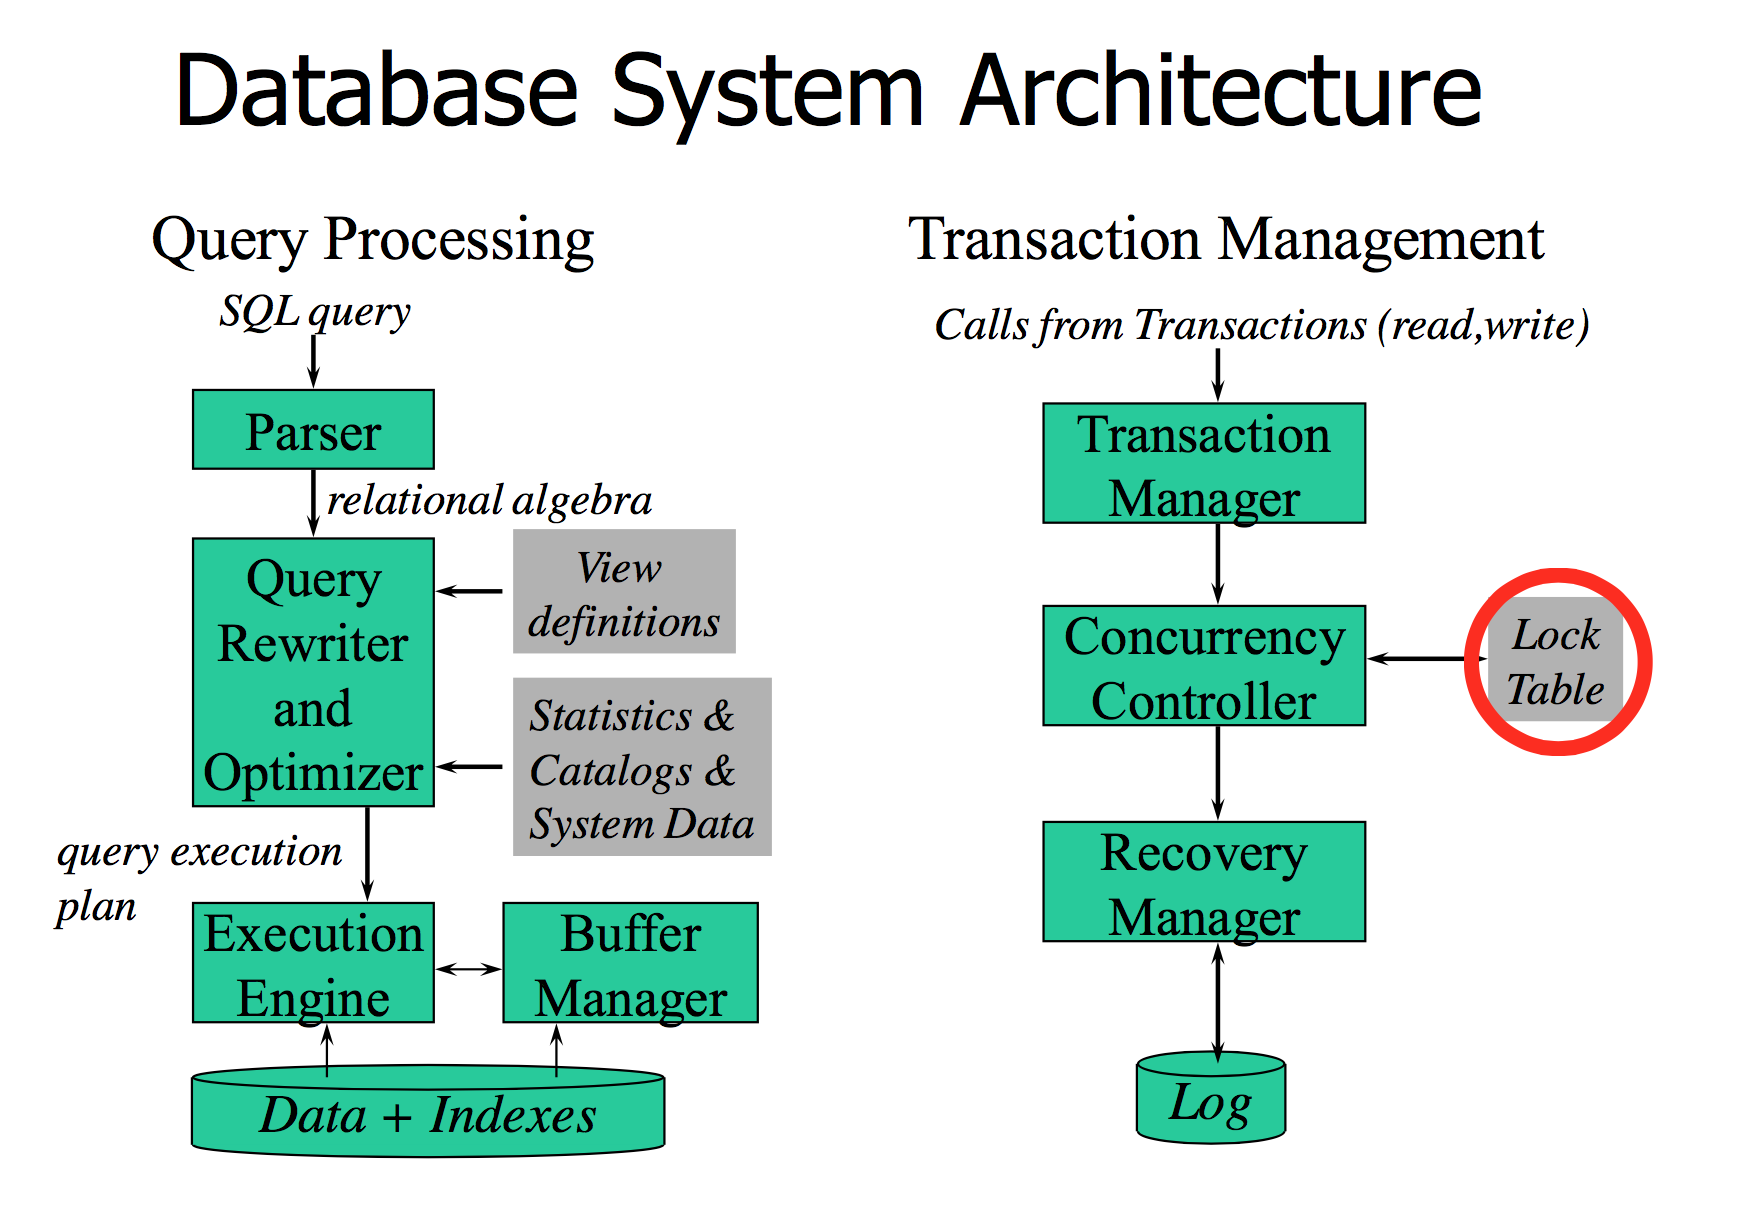
\includegraphics[height=2.2in]{img/db_sys_arch}}
\caption{Database System Architecture}
\label{fig:LABEL}
\end{figure}
\end{itemize}


\chapter{Hardware}
\begin{itemize}
\item Memory Hierarchy 
\begin{enumerate}
\item Blocked-based access 
\item Different Rates of Improvement 
\end{enumerate}
\item Tuned for blocks: Two-Phase, Multiway \textbf{MergeSort} (TPMMS). 
\begin{enumerate}
\item Phase 1: Load db and sort into multiple lists 
\item Phase 2: Merge multiple lists 

Upper data size: 
$$
\frac{M^2}{B}
$$
, where $M\trieq$ RAM byte size, $B\trieq$ block byte size (rather than \#blocks).

\textbf{Core clues}
\begin{enumerate}
\item Phase 1 constraint: max list size: $M$
\item Phase 2 constraint: max \#lists: $\frac{M}{B}$

Thus max data size: $\frac{M^2}{B}$. 
\end{enumerate}

Block I/O cost:
\begin{enumerate}
\item phase 1: $B(R)$ read + $B(R)$ write 
\item phase 2: $B(R)$ read + $B(R)$ write 
\end{enumerate}
, where B(x) is the number of block. 

Thus total IO costs:
$$
4B(R) 
$$
\end{enumerate}
\end{itemize}


\chapter{Indexing}
\section{Conventional indexes}
\begin{enumerate}
\item Basic index types
  \begin{enumerate}
  \item Primary index
  \item Secondary index. 

  Notice the order of index: $i+1, i$ level of indexes. Secondary is at the outer level. Secondary is meaningless to have a dense index. 
  
  
  
  \end{enumerate}
  $\bot$
  \begin{enumerate}
  \item Dense Index
  \item Spare Index: only works on sorted key. 
  \end{enumerate}
\item Multi-level indexes
\item Operations on conventional index
  \begin{enumerate}
  \item Duplication
  \item Deletion
  \item Insertion
  \end{enumerate}
\item Secondary Indexes
  \begin{enumerate}
  \item Non-sequencing \& multi-level
  \item Duplicate values
  
  Solutions:
    \begin{enumerate}
    \item multiple index ptrs
    \item variable size of index list 
    \item chaining records 
    \item bucket (most used)
    \end{enumerate}
  \end{enumerate}
\end{enumerate}
\section{B+Tree}
\subsection{Basics}
\textbf{Root} node can be any size. While \textbf{non-root} nodes have most $n$ slots.

\begin{tabular}{lll}
\hline\noalign{\smallskip}
\textbf{Attrs} & \textbf{Non-leaf} & \textbf{Leaf} \\
\noalign{\smallskip}\hline\noalign{\smallskip}
\textit{Ptrs} & \lceil\frac{n+1}{2}\rceil & \lfloor\frac{n+1}{2}\rfloor \\
\noalign{\smallskip}\hline\noalign{
\caption{Non-root bodes at least half-full}
\end{tabular}

\begin{itemize}
\item Follow the range convention of $[a, b)$.
\item Left leaning convention 
\item \textbf{Ptrs} is different \textbf{slots}. 
\begin{enumerate}
\treeitem Non-leaf keys: slots = ptrs $-1 = \lceil\frac{n+1}{2}\rceil -1$
\treeitem Leaf keys: slots = ptrs $= \lfloor\frac{n+1}{2}\rfloor$
\end{enumerate}
\end{itemize}
\newpage
\subsection{Insertions}
\textbf{Core clues}:
\begin{enumerate}
\item \textbf{Split invariant}: children balanced or left-leaning
\item \textbf{Split}: split half, thus invariant.
\item \textbf{Leaf-Up}: \textit{no delete}, recursively move up the right node's first child; thus invariant.
\item \textbf{Nonleaf-Up}: \textit{delete} and recursively move up the left's last if left-leaning or right's first if balanced; thus invariant. 
\end{enumerate}
\begin{figure}[hbtp]
\centering
\subfloat{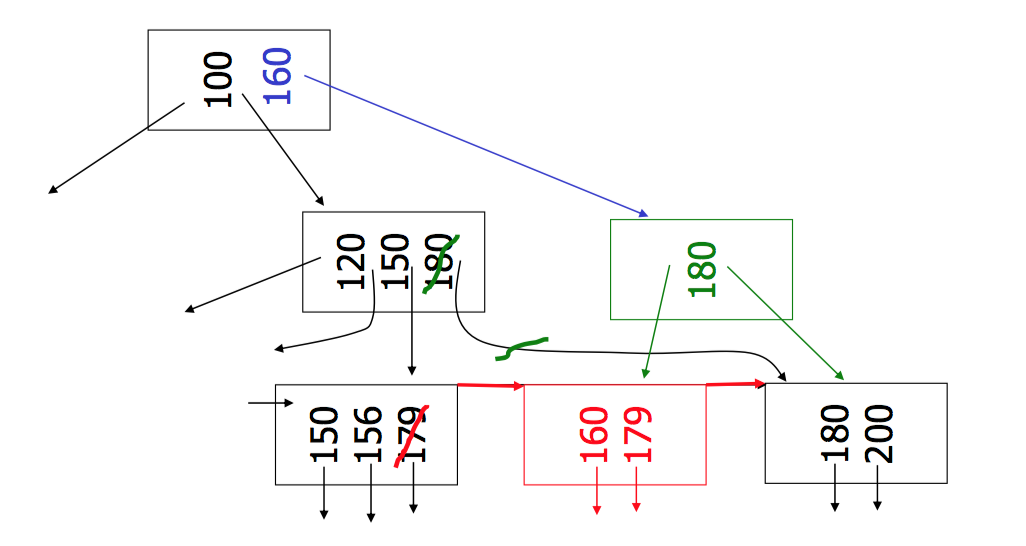
\includegraphics[scale=.70]{img/btreeInsert}}
\caption{B-tree insert, non-leaf up. n=3}
\label{fig:btreeDelete}
\end{figure}
\subsection{Advanced insertions}
Insert a list of sorted keys. 
\begin{itemize}
\item As \textbf{empty} as possible: reverse the order of insertion simply.
\item As \textbf{full} as possible:
reverse engineer the full B-tree. 
\begin{enumerate}
\item Full nodes can only be resulted from insertion rather than splitting
\item Full nodes can be split to $\lceil\frac{n+1}{2}\rceil$ and $\lfloor\frac{n+1}{2}\rfloor$, if left-leaning. 
\item Full nodes can be resulted from inserting the tail node with $\lfloor\frac{n+1}{2}\rfloor$.
\end{enumerate}
Therefore, the the reverse engineer process is:
\begin{enumerate}
\item Reverse insertion on each full leaf nodes, usually the last key. 
\item Reverse splitting result $\lceil\frac{n+1}{2}\rceil$$\lfloor\frac{n+1}{2}\rfloor$ to the original tail nodes of $\lfloor\frac{n+1}{2}\rfloor$. 
\end{enumerate}
\end{itemize}

\subsection{Deletion}
\textbf{Cire clues}:
\begin{enumerate}
\item \textbf{Invariant}: children $\lceil\frac{n+1}{2}\rceil, \lfloor\frac{n+1}{2}\rfloor$
\item \textbf{Fuse}: fuse remaining to left sibling, if left not full. \textit{Delete} upper level. 
\item \textbf{Redistribute}: Extract the last key of left sibling, if left full. \textit{Adjust} upper level.
\item \textbf{Non-leaf fuse}: fuse remaining to left sibling, if left not full. \textit{Move down} the upper level. 
\end{enumerate}
\begin{figure}[hbtp]
\centering
\subfloat{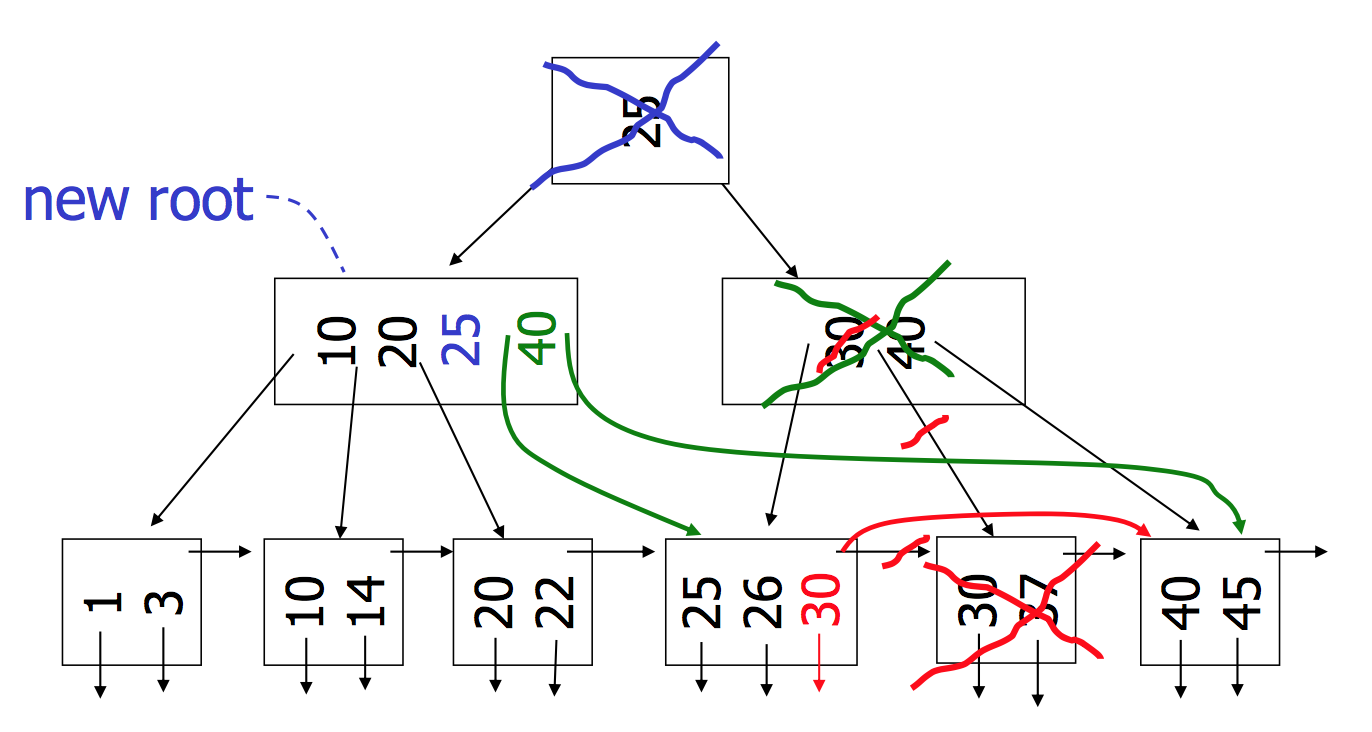
\includegraphics[scale=.60]{img/btreeDelete}}
\caption{B-tree delete, non-leaf fuse/coalese. n=4}
\label{fig:btreeDelete}
\end{figure}
\section{Hash}
\subsection{Extensible hashing}
Core clues:
\begin{enumerate}
\item Number of \note{higher} order bit used $i$: $hash[:i]$ - \textbf{110}001
\item When overflow:
  \begin{enumerate}
  \item \textbf{Expand} the index $i=i+1$.
  \item \textbf{Split} the bucket. Reorganized the split bucket according to new $i$.
  \item \textbf{Untouched} buckets remain untouched. 
  \end{enumerate}
\item Shorthand notation: 110 \framebox{3} K I
\end{enumerate}
\begin{figure}[H]
        \centerline{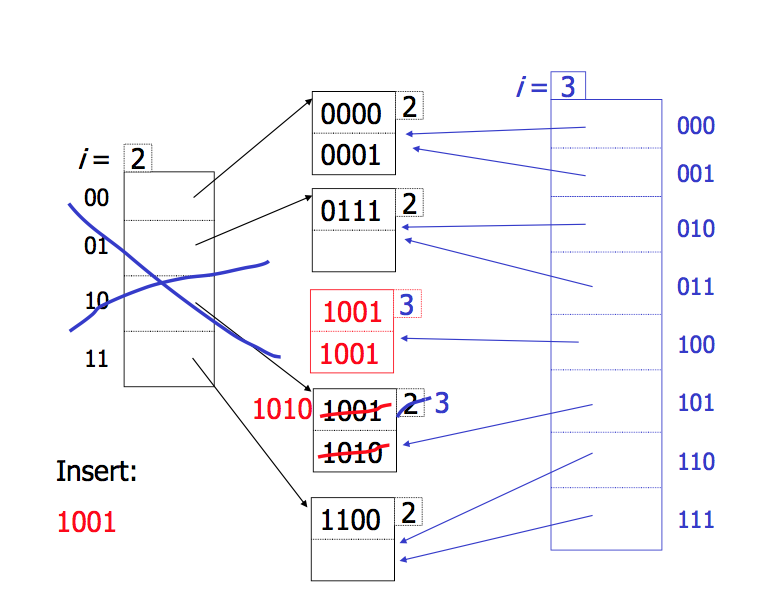
\includegraphics[height = 2in]{img/extensible_hashing}}
        \caption{Extensible Hashing}
    \label{fig:extensibleHashing}
\end{figure}
Initial state of extensible hashing: $i=0$, index $\phi$, 1 ptr to a single block. After $i=1$, index entry $0, 1$; 2 ptrs. 
\subsection{Linear Hashing}
Extensible hashing is exponentially expanding the index; while linear hashing  linearly. 
\begin{figure}[H]
    \centerline{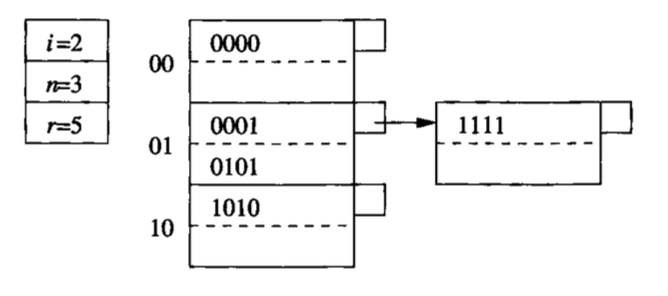
\includegraphics[height = 1in]{img/linearhashing}}
    \caption{Linear Hashing}
  \label{fig:linearHashing}
\end{figure}
\begin{figure}[H]
    \centerline{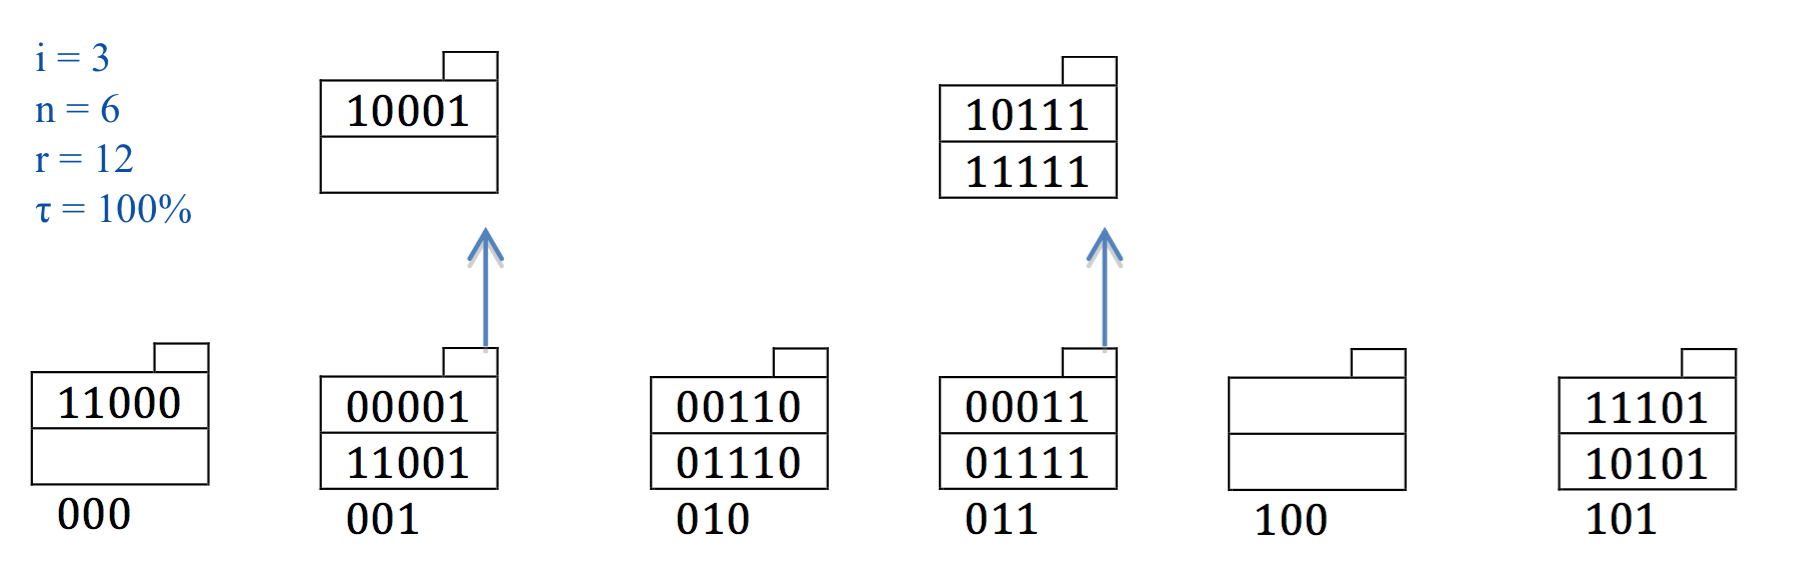
\includegraphics[height = 1.5in]{img/linearHahsing2}}
    \caption{Linear Hashing, overflow ptrs}
  \label{fig:linearHashing2}
\end{figure}
Definitions:
\begin{itemize}
\treeitem $m \triangleq a_1a_2...a_i$, the $i$ \note{lower} bits of $H(K)$ intended for hashing - 110\textbf{001}
\treeitem $n$ number of buckets (blocks) currently using (max number); doesn't count overflow block. 
\treeitem $r$ number of records
\treeitem $\tau$ threshold for $\frac{r}{n\cdot cap}$, where $cap$ is the number of slots per bucket (textbook is $\frac{r}{n}$).
\end{itemize}
Insert: 
\begin{itemize}
\item if $m<n$, insert at $m$-th bucket.
\item if $n\leq m < 2^i$, insert at $0a_2...a_i$-th bucket, (unset the \textit{highest} bit of usage bit $m$).
\item if designated bucket full, append to overflow block. 
\end{itemize}
Expand:
\begin{itemize}
\item if $\frac{r}{n\cdot cap}>\tau$, inc $n$ $\wedge$ if the resulting bucket idx is like $1.*$, split the corresponding $0.*$ bucket. 
\item if $2^i<n$, inc $i$. Bucket idx remain unchanged. ($i$ can be passively derived from $n$) 
\end{itemize}

\section{BitMap}
\begin{figure}[H]
\centering
\subfloat{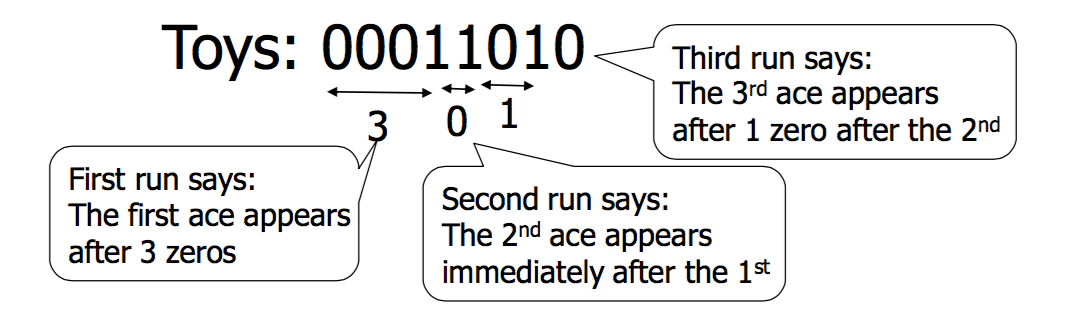
\includegraphics[scale=.80]{img/bitmap}}
\caption{Bitmap}
\label{fig:LABEL}
\end{figure}
Non-encoded bitmap vs. encoded bitmap. 
\\
Core clues:
\begin{enumerate}
\item Gap count of 0's between 1's
\item Encode length information [1]*(i-1)+[0], where i is number of bit for the gap count.
\item Checksum: len info and gap count are of same size
\end{enumerate}
Complexity: 
\begin{align*}
& \sim m \frac{n}{m} 2\log\Big(n/\frac{n}{m} \Big) \\
& \sim n \cdot 2\log m 
\end{align*}
Derivations:
\begin{itemize}
\item $n = T(R)$, $m = V(R, A)$
\item Assume 1's evenly distributed 
\item $\frac{n}{m}$ 1's for each bitmap (i.e. $\frac{\#1's}{unc\ bitmap}$).
\item For an unc bitmap: n-bit length with $\frac{n}{m}$ 1's; $\ra$ run is $\frac{n}{n/m}=m$, (precisely should consider the space taken by 1's), assuming 1's are evenly distributed. $\frac{n}{n/m}$ is \#0's preceding each 1. 
\item For a comp bitmap: $\frac{n}{m}$ 1's with each run $m$, thus encoding length : $\frac{n}{m} 2 \log m$
\item Thus, in total: $m \cdot \frac{n}{m} \cdot 2 \log{m} = 2n\log m$
\end{itemize}

To summarize: 
$$
\#bitmaps \cdot \#1's\in bitmap_i \cdot 2\log\Big(\overline{gapLen\in 0's}\Big)
$$


\chapter{Query Processing}
\section{Basic query processing}
\subsection{Relational algebra}\label{rlsAlgebra}
Notations:
\begin{enumerate}
\item $\sigma$: Selection, \textit{where} (conditions). Selection does not preserver index.
\item $\times$: Cartesian product, \textit{from} product. It does not de-dup columns.  
\item $\Pi$: Projection, \textit{select} (attributes)
\item $x\ra y$: Extended projection, rename $x$ to $y$. Scalar func: $a+b\ra y$, String ops: $c||d \ra y$

\textbf{Scalar} functions: their input comes from the same tuple (as opp. \textbf{aggregate}). 

Notice that $\Pi_{x\ra y} R$ is to project R to x first and to apply the transformation; thus only column $y$ remains. 
$$
\Pi_{x, y\ra z, x+y\ra w} R
$$
Alternatively, $PLUS_{x, y\ra z}$; similarly $CONCAT, MULT, CONCAT}$. Alternative notations for extended projection
\item $\bowtie$: Natural join: $R\bowtie S = \Pi_{distinctAttrs}\sigma_{condOnBoth}(R\times S)$. Notice that the $\times$ is \textbf{bag} version; and $\bowtie$ de-dups \textit{columns}. The results $LHS\equiv RHS$, but the query plans of $LHS, RHS$ may be different. 

\item $\bowtie_{\theta}$: $= \sigma_{\theta} (R\times S)$. $\theta$ is a condition. Notice that, strictly, $\bowtie_\theta$ is \textit{not} the $\theta$ version of natural join, but the $\theta$ version of Cartesian product. It does \textit{not} de-dup \textit{columns}.
However, we usually treat $\bowtie_\theta$ as $\bowtie$, the natural join. 
\item $\gamma$: Group and aggregation

\textbf{Aggregate} functions. 
$$
\gamma_{attr_{grpby}, aggrFn(attr) \ra attr'}
$$
Alternatively, $SUM_{attr_{grpby},aggrFn(attr)\ra attr'}$, similarly $AVG, MIN, MAX, COUNT$. Alternative notations for group and aggregation. 
\item $\tau$: Order by. 

A result $o(exp)$ is ordered if
\begin{enumerate}
\item $o$ \textbf{retains} the originally ordered $exp$. (e.g. $\sigma$)
\item $o$ \textbf{creates} ordering. (e.g. ordered by pk, then iterative joining implt with FLY)
\end{enumerate}
$\sigma$ may retain the order generated by $\tau$ but depends on implementation. e.g. $\sigma^\text{FLY}$ may prodeces a ordered result. Discussion: 

$$
\tau_{R.A, R.B}\ \sigma_{R.B>5}^\text{FLY} R
$$
\begin{flushright}, produces a list\end{flushright}
$$
\sigma^\text{FLY}_{R.B>5}\ \tau_{R.A, R.B} R 
$$
\begin{flushright}, produces a bag but preserves the order.\end{flushright} 
\end{enumerate}
\subsection{Query Plan}
A simple SFW (Select From Where). 
\begin{enumerate}
\item Naive plan p:
$$
\Pi_{attr_1,attr_2}^\text{FLY}\Big[\sigma_{cond_R\wedge cond_S\wedge cond_{RS}}^\text{FLY} (R^\text{SCAN}\times S^\text{SCAN})\Big]
$$

FLY and SCAN are how exactly the plan is run.
\begin{enumerate}
\item \textbf{FLY}: on the fly, one entry at a time. Implementation: Iterator. No intermediate storage 
\item \textbf{SCAN}: scan the tables, one block at a time.
\begin{enumerate}
\item \textbf{Table-scan}. operator simply reads each block holding tuples of the relation.
\item \textbf{Index-scan}. uses an index to find tuples
\item \textbf{Sort-scan}. produces the tuples in sorted order.

\end{enumerate}}
\end{enumerate}

\item Join Plan (plan II):
$$
\Pi_{attrs} \Big[(\sigma_{cond_R}R)  \bowtie^\text{HASH} (\sigma_{cond_S}S) \Big]
$$
\item Index plan (plan III):

$$
\Pi_{attrs}\ \sigma_{cond_S}(\sigma_{cond_R}^\text{INDEX}R \bowtie^\text{RI} S)
$$
$\bowtie^\text{RI}$ Right Index Join. 
Steps:
\begin{itemize}
\item $\sigma^{\text{INDEX}}$ uses index to get tuples based on condition on $R$. 
\item $\bowtie^\text{RI}$. For each tuple in the result $R$:
\begin{itemize}
\item Match $S$'s tuple using $S$'s index, in $O(1)$. 
\end{itemize}
\item $\sigma$ filters $S$ based on condition on $S$.
\item $\Pi_{attrs}$ ...
\end{itemize}
\end{enumerate}
\section{From query to optimal plan}
\begin{enumerate}
\item \textbf{lqp}. logical query plan $\equiv$ algebra ops 
\item Algebraic rewritings to transform the lqp
\item Physical Plan
\item Example:
\begin{itemize}
\item \textbf{``IN'' Elimination}: 
\begin{pseudo}
select A.a
from A where A.v in (
    select B.v from B where cond_b
);
\end{pseudo}
IN is transformed into $\sigma (A\times B)$. Then the basic algebra is:
$$
\Pi_{A.a}\ \sigma_{A.v=B.v}\ (A \times \Pi \sigma B)
$$
further optimized:
$$
\Pi_{A.a}(A \underset{A.v=B.v}\bowtie \Pi \sigma B)
$$
\item \textbf{``NOT IN'' Elimination}:
$$
\Pi_{A.a} [A - \sigma_{A.v=B.v} (A\times \Pi\sigma B)]
$$
further optimized:
$$
\Pi_{A.a}[A-A\underset{A.v=B.v}\bowtie \Pi\sigma B}]
$$

\end{itemize}
\end{enumerate}
\section{Bag algebra, list algebra, and extensions}
In this nodes, bag-version operations are assumed. 
\begin{enumerate}
\item $\cup, \cap$: Algebraic Operators (Bag Version)
$$
R\cup S
$$
\item $\delta$: Convert to set (DISTINCT)
$$
\delta(R)
$$
\item Extended relational algebra - Section \ref{rlsAlgebra}.
\end{enumerate}
\section{Relational algebra optimization}
\subsection{Rewriting}
\begin{enumerate}
\item \rih{Commutativity and Associativity}
\begin{align*}
R \cdot S &= S\cdot R \\
R\cdot (S\cdot T) &= (R\cdot S) \cdot T \\
\end{align}

, where $\cdot \in \{\times, \bowtie, \cup, \cap \}$  

proof: $R\times S = S\times R$
\begin{align*}
& R \times S \subset S \times R \\
& R \times S \supset S \times R \\
& \forall t, t\in R\times S,\mbox{ n times} \\
& r \in R\mbox{ m times}, s\in S \mbox{ k times}\\
& n = m*k \\
& \Ra\mbox{ find corresponding }t \in sr, k*m,\mbox{ n times} \\ 
& \therefore R \times S \subset S \times R \\
& \mbox{vice versa...}
\end{align*}
\item \rih{Logics}
\begin{align*}
\sigma_{c_1\wedge c_2}R &= \sigma_{c_1}\ \sigma_{c_2}R \\
\sigma_{c_1\vee c_2}R &= \sigma_{c_1}R\ \cup\ \sigma_{c_2}R
\end{align*}
\begin{flushright}, notice that $\vee$ only applies for \note{set} version\end{flushright}
To apply $\vee$ to \note{bag} version: 
\begin{align*}
\sigma_{c_1\vee c_2}R = \sigma_{c_1} R\ \cup\ \sigma_{c_2} (R-\sigma_{c_1}R)
\end{align*}

On $\vee$ on $\bowtie$, where $c_1$ on $R$ and $c_2$ on $S$.
\begin{align*}
\sigma_{c_1 \vee c_2} R\bowtie S &= \sigma_{c_1} R \bowtie S\ \cup\ (R-\sigma_c_1 R)\bowtie \sigma_c_2 S \\
&= \sigma_c_2S \bowtie R\ \cup\ (S-\sigma_c_2 S) \bowtie \sigma_c_1 R
\end{align*}

Decomposition of Negation:
\begin{align*}
\sigma_{\neg c_1} R &= R - \sigma_{c_1} R \\
\sigma_{c_1 \wedge \neg c_2}R &= \sigma_{c_1} R - \sigma_{c_2} R \\
\sigma_{c_1 \vee \neg c_2}R &= \sigma_{c_1} R\ \cup\ \sigma_{\neg c_2} (R-\sigma_{c_1}R)\\ &= \sigma_{c_1} R\ \cup\ (R-\sigma_c_1 R) - \sigma_c_2(R-\sigma_c_1 R)
\end{align*}

\item \rih{Push down $\sigma$} !important
\begin{itemize}
\item General
$$
\sigma_{c}(R\cdot S) = (\sigma_{c} R)\cdot (\sigma_{c} S) 
$$
\begin{flushright}, where $\cdot\in \{-, \cup, \times, \bowtie\}$. \end{flushright}

\item For $\{-\}$, it can directly drop the selection: $\sigma_{c}S$ to $S$. 
$$
\sigma_{c}(R-S) = (\sigma_{c} R)-S
$$
\item For $\{\times, \bowtie\}$, it can further drops the $\sigma_{c}T$ to $T$ if the condition does \textit{not} refer to attributes in $T$.
\begin{align*}
\sigma_{c}(R\cdot S) = R\cdot (\sigma_{c} S) 
\end{align*}
\end{itemize}

Proof: $\sigma_{A=2}(R\bowtie S) = (\sigma_{A=2}R)\bowtie S$, given commutativity and $\sigma_{c}(R\bowtie S) = R\bowtie \sigma_{c}S$
\begin{align*}
\sigma_{A=2}(R\bowtie S) = \sigma_{A=2}(S\bowtie R) = S \bowtie (\sigma_{A=2}R)=(\sigma_{A=2}R\bowtie S)
\end{align*}
This is a technique of proof by using axioms. 

\rih{Combine $\pi$ \& $\sigma$}

\item \rih{Push down $\pi$ - Supperset $\pi$} 
 
\begin{align*}
& \pi_x (R \cup S) = \pi_x R \cup \pi_x S \\
& \pi_x (R\cap S) \neq \pi_x R \cap \pi_x S\\
& \pi_x (R-S) \neq \pi_x R - \pi_x S\\
& \pi_a (R \times S) = \pi_a (\pi_{c_1 \supseteq a}R \times \pi_{c_2 \supseteq a} S) \\
& \pi_a (R \bowtie S) = \pi_a(\pi_{c_1 \supseteq (a \cup R.c)}\ R \bowtie \pi_{c_2 \supseteq (a\cup S.c)}\ S) \\
& \pi_x R = \pi_x \pi_{y\supseteq x} R
\end{align*}
\begin{itemize}
\item Supperset for conditions in $\pi$.
\item $\pi$ can reduce the length of a tuple; thus it is useful to push down $\pi$ to fit more tuples in memory. When denoting $\supset, \supseteq, \subset, \subseteq$, it is for AND composite. $cond1\supseteq a$ is a shorthand notation for $\{c_1|c_1 \supseteq a\}$, a notation for superset. 
\item \rih{Difference}. Notice that, $\pi_a (R-S) \neq \pi_a R - \pi_a S$ 
\item \rih{Push down priority of $\pi, \sigma$}. Normally $\sigma$ is given higher priority than $\pi$ if $\sigma$ can do index selection to avoid $\pi$ on all tuples (Section - \ref{sec:queryExec})
\end{itemize}
\item \rih{Aggregation} 

\begin{align*}
& \text{Push down } \sigma\\
& \sigma_{c\subset grpAttrs} \Sigma_{grpAttrs; attr\ra attr'} R = \Sigma_{grpAttrs, attr\ra attr'} \sigma_{c\subset grpAttrs} R \\
& \text{Push down } \gamma\\
& \Sigma_{GL;GA\ra RA} (R \cup S) = +_{RA1, RA2:RA} (\Sigma_{GL; GA\ra RA1 }R \bowtie \Sigma_{GL; GA\ra RA2} S)\\
& \text{Combine } \gamma\\
& \Sigma_{GL2; RA1 \ra RA2} \Sigma_{GL1; GA \ra RA1} R = \Sigma_{GL2; GA\ra RA2} R
\end{align*}
Notation, in slides it is $grpList$ or $GL$ as $grpAttrs$; $SUM$ as $\Sigma$; $PLUS$ as +.
\item \rih{Cost, rule of thumb} 

\end{enumerate}
\subsection{Proof/Disproof the equivalence of rewriting}
The \note{breakthrough} points: 
\begin{enumerate}
\item $\phi$ table
\item NULL column. 
\item Bag version duplicates
\end{enumerate}



\section{Algorithms for Relational Algebra Operators}
\subsection{Query Execution}\label{sec:queryExec}
\subsubsection{Implementation of $\sigma$}
\begin{enumerate}
\item $\sigma^\text{INDEX}_{A=c}$ 
\begin{eqnarray*}
time = \left\{ \begin{array}{rl}
  \frac{B(R)}{V(R, A)} &\text{// if tuple clustered on $A$, default }\\
  \frac{T(R)}{V(R, A)} &\text{// if tuple not clustered on $A$}
       \end{array} \right.
\end{eqnarray*}
Normally pipelined version of $\sigma^\text{INDEX}_{A=c}$ is impossible 
\item $\sigma^\text{SCAN}_{A=c}$
\begin{eqnarray*}
time = \left\{ \begin{array}{rl}
  B(R) &\text{// if normal }\\
  0 &\text{// if pipeline}
       \end{array} \right.
\end{eqnarray*}
\end{enumerate}
\subsubsection{Implementations of $\bowtie$}

Notice:
\begin{itemize}
\item \textbf{Output pipeline.} Write out of the join result at the end/final/return is not considered due to output pipeline, always.
\item \textbf{Input pipeline.} 1 $B(R)$ may be saved due to input pipeline. 
\item \textbf{Cost model}. Time of execution is measured by number of disk IOs. 
\end{itemize}

$M$ for blocks rather than bytes size. 

\begin{enumerate}
\item $\bowtie^{\text{1P}}$ Iteration join (one pass)

\textbf{Requirement}. As long as any of the two can fit into the memory. 
$$
\min(B(R), B(S)) < M
$$

\textbf{Time}. Load a table to memory, and then loop join, thus
\begin{eqnarray*}
time = \left\{ \begin{array}{rl}
  B(R)+B(S) &\text{// if normal }\\
  0+B(S) &\text{// if pipeline}
       \end{array} \right.
\end{eqnarray*}
\item $\bowtie^\text{SM}$ Merge join (two passes)

\textbf{Process.} Two phases:
\begin{enumerate}
\item Sort-merge phase. \textbf{Mem} req: $|R|/M<M; |S|/M<M $
\item Merge-join phase. \textbf{Mem} req: $|R|/M+|S|/M <M$

Thus, all sqrt can fit into memory. 
$$
M>\sqrt{\max{(|R|,|S|)}}
$$
\end{enumerate}

, where $|X|\triangleq B(X)$

Possible to combine the merge 

\textbf{Time.} \textbf{Sort}: 1 read 1 write. \textbf{Merge}: 1 read; thus 
\begin{eqnarray*}
time = \left\{ \begin{array}{rl}
  3B(R)+3B(S) &\text{// if normal} \\
  B(R)+3B(S) &\text{// if $R$ sorted on attr} \\
  2B(R)+3B(S) &\text{// if input pipeline on $R$}\\
  0+3B(S) &\text{// if input pipeline on $R$ and $R$ sorted}
       \end{array} \right.
\end{eqnarray*}
Multiple times of $\bowtie^\text{SM}$, but may not sorted on the same attr. 
\item $\bowtie^\text{RI}, \bowtie^\text{INDEX}$ Index join 

\textbf{Difference.} btw RI and INDEX: $\bowtie^\text{RI}$ uses only 1 index; while $\bowtie^\text{INDEX}$ uses 2 indexes, thus it can process on indexes first (ptr), delaying the block access to data. 

\textbf{Time \& Mem.} when \textit{no} relation fits in mem, $\bowtie^{RI}$ outperforms $\forall$ any other technique, even for 1Pass.  

\textbf{Cost}. It reads $B(R)$; for each $T(R)$, loads $\lceil B(S)/V(S, B)\rceil$ blocks according to the index; thus 
\begin{eqnarray*}
time_\text{clustedIndex} = \left\{ \begin{array}{rl}
  B(R)+T(R)\cdot \frac{B(S)}{V(S, B)} &\text{// if normal} \\
  T(R)\cdot \frac{B(S)}{V(S, B)} &\text{// if input pipeline}\\
       \end{array} \right.
\end{eqnarray*}
\begin{eqnarray*}
time_\text{scatteredIndex} = \left\{ \begin{array}{rl}
  B(R)+T(R)\cdot \Big(1+\frac{T(S)}{V(S, B)}\Big) &\text{// if normal} \\
  T(R)\cdot \Big(1+\frac{T(S)}{V(S, B)}\Big)} &\text{// if input pipeline}\\
       \end{array} \right.
\end{eqnarray*}
If index or sorted on common attr R.C, de-duplication possible; thus change
$$
T(R) \ra V(R)
$$
\begin{itemize}
\item $1+...$, the 1 for \textit{index block access} to the non-cached leaf nodes of the B-tree index 
\item Create index (normally already created): read blocks and write index $B(S)+B(index)$
\item $\sigma^{\text{RI}}$ will pay off when $B(S)$ and $V(S,B)$ are gigantic. 
\end{itemize}
\item $\bowtie^\text{HASH}$ Hash join 

\textbf{Requirement.} $\min\big(B(R_{i}), B(S_{i}})\big) <M$. The smaller \textit{bucket} need to fit in mem when join the bucket. There are $M-1$ buckets $R_i, S_i$, thus
\begin{align*}
M &\geq \frac{\min(|R|, |S|)}{M-1} \\
M &> \sqrt{\min(|R|, |S|)}
\end{align*}

\textbf{Process.} Two phases
\begin{enumerate}
\item Hash every tuple into $M-1$ buckets $R_i, S_i$ (the remaining 1 for the temp working memory).
\item Load either bucket $R_i, S_i$ into mem, scan the other and join.
\end{enumerate}
\textbf{Cost.} To create hashed buckets, 1 read write R, S. To hash join, 1 read; thus 
\begin{eqnarray*}
time = \left\{ \begin{array}{rl}
  3B(R)+3B(S) &\text{// if normal} \\
  2B(R)+3B(S) &\text{// if input pipeline on $R$}\\
       \end{array} \right.
\end{eqnarray*}
Hash join is similar to sort-merge join. 
\end{enumerate}

\subsubsection{Analysis}
\begin{enumerate}
\item \textbf{Output pipeline.} Results are \textit{pipelined} to output, thus not consider write the final result into disk. 
\item \textbf{Sort.} Sorted table does not need to sort in sort-merge on the sorted attr.
\begin{enumerate}
\item 1-pass on sorted table, result may also be sorted (depends).
\item sort-merge will produce sorted result
\end{enumerate}
\item \textbf{Intermediate non-index.} Intermediate results do not have index; unless otherwise stated.  
\item \textbf{Cost algorithm.} calculate time $\leftarrow$ calculate the \# disk IO $\leftarrow$ \# blocks $B(R)$ $\leftarrow$ intermediate tuple size $T(R)$. 
\end{enumerate}
\subsection{Cost analysis (intermediate size)}
\rih{Intro}
\begin{itemize}
\item Two aspects of cost analysis:
\begin{enumerate}
\item Size of the intermediate result 
\item Number of IOs.
\end{enumerate}
\item Notations
\begin{enumerate}
\treeitem T(R) : #tuples in R
\treeitem S(R) : #bytes (size) in each R tuple
\treeitem B(R): #blocks to hold all R tuples 
\treeitem V(R, A) : #distinct values in R for attribute A
\end{enumerate}
\item Corner case 
$$
V(R_1\times R_2) \approx V(R_1, A)
$$
Corner case: $R_2=\phi$, then RHS should be 0. But, in size estimation, doesn't consider the corner case. Normally, only the average case (uniform distr.) is considered. 
\end{itemize}
\rih{Size estimation for $\bowtie$}
\begin{itemize}
\item Assumption: either $\pi_{A}R_1 \subseteq \pi_{A}R_2$ or $\pi_{A}R_1 \supseteq \pi_{A}R_2$.
Notice the assumption may be violatd. 
\item \textbraceleft PK, FK\textbraceright\ relationship $R_1\bowtie R_2$

One way PK, FK for $R_1, R_2$: 
$$
T(W) = \frac{T(R_1)}{V(R_1, A)} T(R_2)
$$

Generalized to symmetry (this is an est.): 
$$
T(W) = \frac{T(R_1)T(R_2)}{\max\{V(R_1, A), V(R_2, A)\}}
$$
\end{itemize}
\rih{Subexpressions \& Value preservation}

\textbf{Probability approach}. The combination should not change the a $V$'s prob distr. since assumped indpt; thus,\begin{itemize}
\item Value preservation for the pushing down of $\sigma$. 
\item Value preservation for the composite $\bowtie$. 
\end{itemize}
\subsection{Plan Enumeration}
\subsubsection{Hypergraph}
INGRES \textit{greedy} heuristic search. 

Small relation $\triangleq \sigma R$  

Two assumptions:
\begin{enumerate}
\item $\forall$ join attr, index on it
\item $\exists$  small reations
\end{enumerate}
Left-deep algebraic expression.
\subsection{Analyze query processing}
Process:
\begin{enumerate}
\item Relationship hypergraph for visualization. 
\item Preprocess memory inforamtion 
\item Def shorthand notations for conditions. 
\item Draw the parse tree. 
\item Calculate $B(.), T(.)$, tuple per block alternately. Notice $S(.)$ affects tuple per block. 

Given $R$ is $a$ tuples per block, $S$ is $b$ tuple per block. Then $R\bowtie S$ is $$
\frac{1}{\frac{1}{a}+\frac{1}{b}} 
$$
per block. 
\end{enumerate}
\chapter{Failure Recovery (FR)}
\section*{Introduction}
Consistency. T executes 1) until completion \& 2) in isolation. 

Violation of consistency: 
\begin{enumerate}
\item Until completion: failures - Failure Recovery (FR)
\item In isolation: concurrent control with data sharing - Concurrency Control
(CC)
\item Intersection of both - FR $\cup$ CC
\end{enumerate}

\section{Notations}
Block based 
\begin{enumerate}
\treeitem Input(x) $\triangleq$ part mem := x with block 
\treeitem Output(x) $\triangleq$ block := x with block
\treeitem Read(x,t) $\triangleq$ t := x in block 
\treeitem Write(x,t) $\triangleq$ x in block := t // write need Input(x) since block based access.
\end{enumerate}

\section{FR Solutions}
\subsection{Undo logging}
Immediate write db data to disk 
\subsubsection{Clues}
To undo, records: 
\begin{enumerate}
\item \textbf{start}: $<T_i, \text{start}>$
\item \textbf{prior values}: $<T_i, A, \text{prior}>$
\item \textbf{commit}: $<T_i, \text{commit}>$
\end{enumerate}

\subsubsection{Undo logging rules}
\begin{enumerate}
\item \unibox{\textbf{Log record on disk \note{BEFORE} correspondence}}: before x is modified on disk, log records pertaining to x must be on disk
\item \unibox{\textbf{Commit log on disk \note{AFTER} all}}: before commit is flushed to log, all (not any) writes of $T$ must be reflected on disk.
\end{enumerate}

\newpage
\subsubsection{Recovery rules}
Backward pass

Process:
\begin{pseudo}
$S = T_i$ with start $\wedge$ ($\neg$ commit $\vee$ $\neg$ abort)
foreach record $T_i, X, x$ reversed=true
  if $T_i \in S$
    write(X, x) 
    output(X)
foreach $T_i$
  log $T_i, abort$
\end{pseudo}
Failure during recovery is not an issue, since undo logging is idempotent.



\subsection{Redo logging}
Deferred write db data to disk. 
\subsubsection{Clues}
To redo, records: 
\begin{enumerate}
\item \textbf{start}: $<T_i, \text{start}>$
\item \textbf{posterior values}: $<T_i, A, \text{posterior}>$
\item \textbf{commit}: $<T_i, \text{commit}>$
\end{enumerate}

\subsubsection{Redo logging rules}
\begin{enumerate}
\item \unibox{\textbf{Log record on disk \note{BEFORE} correspondence}}: before x is modified on disk, log records pertaining to x must be on disk
\item \unibox{\textbf{Commit log on disk \note{BEFORE} any}}: before any (not all) writes of $T$ is reflected on disk, commit must flush to log.
\item \unibox{\textbf{Flush}}: flush log records at $T$ commit. 
\end{enumerate}

\subsubsection{Recovery rules}
Forward pass

Process: 
\begin{pseudo}
# no abort log
$S = T_i$ with start $\wedge$ commit
foreach record $T_i, X, x$ reversed=false
  if $T_i \in S$
    write(X, x)
    output(X) # optional
\end{pseudo}

\subsubsection{Checkpoint}
Redo recovery is very slow. 

\subsection*{Comparison: undo vs. redo }
\begin{enumerate}
\item Undo
\begin{enumerate}
\item unable to bring \textit{backup} DB copies up to date (since no posterior values recorded, need to diff db and backup db).
\item real writes at end of transaction needed (since immediate db write)
\end{enumerate}
\item Redo
\begin{enumerate}
\item need to keep all modified blocks in \textit{memory} until commit (since deferred db write)
\end{enumerate}
\end{enumerate}

\subsection{Undo/Redo logging}
$<T_i, A, \text{posterior}, \text{prior}>$
\subsubsection{Clues}
\begin{enumerate}
\item \textbf{start}: $<T_i, \text{start}>$
\item \textbf{posterior, priror values}: $<T_i, A, \text{posterior}, \text{prior}>$
\item \textbf{commit}: $<T_i, \text{commit}>$
\end{enumerate}

\subsubsection{Undo/Redo logging rules}
\begin{enumerate}
\item \unibox{\textbf{Log record on disk \note{BEFORE} correspondence}}: before X is modified on disk, log records pertaining to X must be on disk
\item \unibox{\textbf{Commit before any/after all}}: no requirement of $X$ modified on disk w.r.t. $T_i$ commit. (i.e. X can be modified on disk before or after commit log).
\item \unibox{\textbf{Flush}}: flush log records at $T$ commit. 
\end{enumerate}

\subsubsection{Recovery rules}
$S = T_i$ with start $\wedge$ commit
\begin{enumerate}
\item \textbf{Backward pass}: last checkpoint $\leftarrow$ end of log; undo $T \notin S$.
\item \textbf{Forward pass}: last checkpoint $\rightarrow$ end of log; redo $T \in S$.
\end{enumerate}

\subsubsection{Checkpoint - Non-quiesce}

\subsection{Summary}
\begin{tabular}{llll}
\hline\noalign{\smallskip}
\textbf{Req.} & \textbf{Undo} & \textbf{Redo} & \textbf{Undo/Redo}\\
\noalign{\smallskip}\hline\noalign{\smallskip}
\textbf{Log record} & before corr & before corr & before corr\\
\textbf{Log commit} & after all & before any & $\phi$\\
\textbf{Flush} & $\phi$ & at $T$ commit & at $T$ commit\\
\noalign{\smallskip}\hline\noalign{\smallskip}
\caption{FR logging}
\end{tabular}

\chapter{Concurrency Control (CC)}
\section{Concepts}
\begin{enumerate}
\item \textbf{Conflict actions}: RW, WR, WW. e.g. RW is $R_i(A); W_j(A)$. Different transactions' action on the same attr. 
\item \textbf{Schedule}: chronological order of actions 
\item \textbf{Serial schedule}: no interleaving actions of transactions in schedule
\item \textbf{Conflict equivalent $\equiv^c$}: $S_1 \equiv^c S_2$ if $S_1$ can be transformed into $S_2$ by swaps non-conflicting actions inter-transactions.
\item \textbf{Conflict serializable}: a schedule $S$ is conflict serializable if $\exists SerS, SerS\text{ is a serial schedule } \wedge S\equiv^c SerS$.
\end{enumerate}

Only non-conflicting actions can be swapped. Unable to swap conflicting actions.


\section{Precedence Graph}
\subsection{Definitions}
Implicitly assume $i\neq j$.

\textbf{Precedes}: $T_i <_S T_j$ in $S$; it is possible $T_j <_{S'} T_j$ in $S'$.

\textbf{Conflict precedes}: $T_i$ precedes $T_j$ in $S$ ($T_i <_S T_j$) with conflict actions. 

Graph definitions: 
\begin{enumerate}
\item $G = P(S)$. A directed graph 
\item $V \triangleq \{T\mid T\in S\}$
\item $E \triangleq \{T_i \ra T_j\mid p_i(A) <_s q_j(A) \wedge p_i(A)  \text{ conflicts } q_j(A)\}$. 
\end{enumerate}
\begin{figure}[hbtp]
\centering
\subfloat{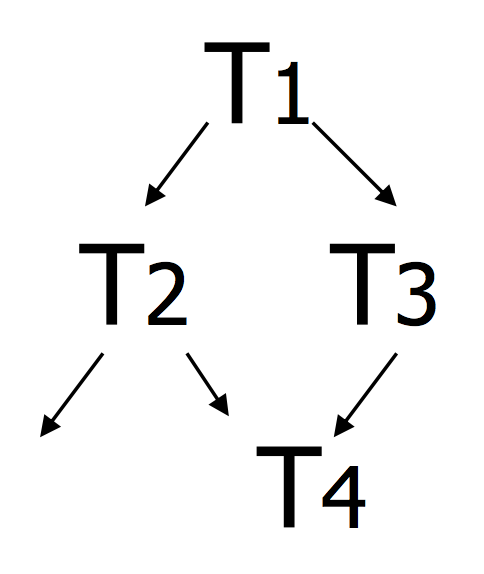
\includegraphics[scale=.40]{img/precdnGraph}}
\caption{Precedence Graph}
\label{fig:precdnGraph}
\end{figure}
To construct a $P(S)$:
\begin{pseudo}
foreach object $A$
  foreach ordered pair $p_i(A), q_j(A)$
    if $p_i(A) \text{ conflicts } q_j(A)$
      add edge $T_i \ra T_j$
\end{pseudo}
\subsection{Theorem}
\begin{enumerate}
\item\ Lemma: 
$$S_1 \equiv^c S_2 \Ra P(S_1)=P(S_2)$$
\item Theorem:
$$P(S) \text{ is acyclic} \Leftrightarrow S \text{ is conflict serializable } \exists serS$$
\end{enumerate}
\section{Lock}
\subsection{Fundamental locking protocol}
\subsubsection{Protocol rules}
3 fundamental rules: 1. Well-formed (attr) 2. Legal ($Ts$) 3. 2PL
\begin{figure}[H]
    \centerline{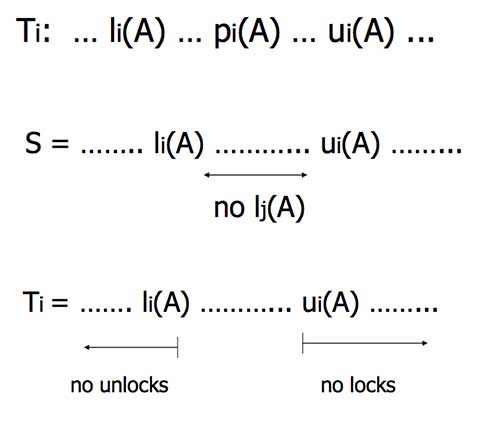
\includegraphics[height = 1.8in]{img/lockFundamental}}
    \caption{Fundamental Locking Protocol: well-formed, legal, 2PL $\Ra$ conflict serializable}
  \label{fig:fundamentalLockingProtocol}
\end{figure}
\begin{enumerate}
\item \textbf{Well-formed}: $\forall$ R/W action. $T_i$ has to lock $l_i(A)$ before the action, and has to unlock $u_i(A)$ after the action.
\item \textbf{Legal}: No $T_j$ can $l_j(A)$ during the time range of $l_i(A) ... u_i(A)$ of $T_i$.
\item \textbf{2PL}: Two-phase lock, For each $T_i$, no $u_i(.)$ before $l_i(.)$ and no $l_i(.)$ after $u_i(.)$. 
\end{enumerate}

2PL may lead to deadlock, thus need to detect deadlock and abort the later transaction.

Strict 2PL: $\forall R_i, W_i, u_i \cdot R_i(.)/W_i(.) <_S u_i(.) $

\subsubsection{Proof}
Prove that: under the 3 rules of the locking protocol $\Ra$ schedules $S$ conflict serializable. 

Lemma: In $S$, 
$$
T_i \ra T_j \Ra SH(T_i) <_s SH(T_j)
$$

, where $SH(T_i)\triangleq Shrink(T_i)$, first unlock action of $T_i$.

Then prove by contradiction using the lemma. 
\subsection{Lock Performance}
\subsubsection{Lock modes}
Lock modes $l\hp \mat{M}$:
\begin{enumerate}
\treeitem \textbf{Shared S}: SS $\neg$ conflict 
\treeitem \textbf{Exclusive X}
\treeitem \textbf{Incremental I}: II $\neg$ conflict 
\treeitem \textbf{Update U}: knows $l\hp S$ will upgrade to $l\hp X$. Avoid upgrade causing deadlock.
\end{enumerate}
Operations:
\begin{enumerate}
\item Upgrade: $l\hp S \ra l\hp X$. Notice upgrade is different from update.
\end{enumerate}
Compatibility matrix: 

compatibility of different modes in \textbf{legal} scheduler.
\begin{figure}[H]
\centering
\begin{tabular}{cc}
  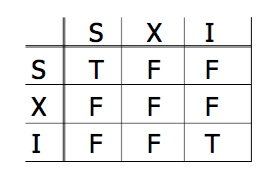
\includegraphics[height = 0.8in]{img/SXI} &
  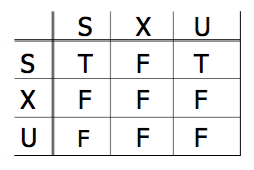
\includegraphics[height = 0.77in]{img/SXU} &
  a & b 
\end{tabular}
\caption{(a) SXI compatibility. (b) SXU compatibility.}
\label{fig:images}
\end{figure}

\subsubsection{Lock Table}
Hash table + LinedList for info.
\begin{figure}[H]
    \centerline{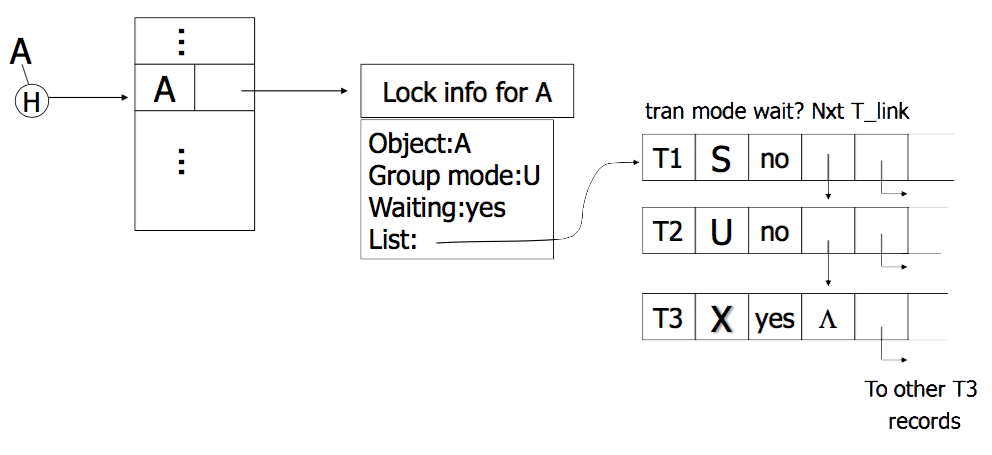
\includegraphics[height = 1.8in, width=3.8in]{img/lockTable}}
    \caption{Lock Table}
  \label{fig:lockTable}
\end{figure}


\subsubsection{Multi-granularity}
The object (lock target) is multi-granular: Relation, disk block, tuple. 

I for \textbf{intent}.

Compatibility matrix:  
\begin{figure}[H]
    \centerline{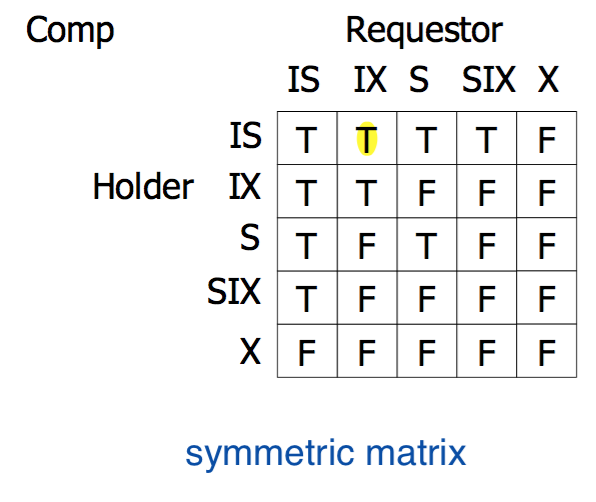
\includegraphics[height = 1.7in]{img/lockModes}}
    \caption{Compatibility Matrix}
  \label{fig:compatibilityMatrix}
\end{figure}

\begin{tabular}{ll}
\hline\noalign{\smallskip}
\textbf{Parent locked in} & \textbf{Child can be locked in} \\
\noalign{\smallskip}\hline\noalign{\smallskip}
IS & IS S \\
IX & all \\
S & [IS S] \\
SIX & IX X [SIX, IS, S] \\
X & none\\
\noalign{\smallskip}\hline\noalign{\smallskip}
\caption{Hierarchy & [.] for not necessary}
\end{tabular}


\subsubsection{Delete and Insert}
\begin{itemize}
\item Delete: lock on tuple
\item Insert: 
\begin{enumerate}
\item Lock on tuple. Issue of phantom objects
\item Lock on table. Issue of concurrency 
\item Lock on partial table by B+Tree index
\end{enumerate}
\end{itemize}


\section{Tree-based CC}
\subsection{Clues}
Once the child has been locked, the $\pi$ can be unlocked
\subsection{Rules}
Tree protocol rules for $X$ 
\begin{enumerate}
\item 1st lock by $T_i$ can be on any item 
\item Subsequently, item Q can be locked by $T_i$ only if $\pi(Q)$ is locked by $T_i$.
\item Item can be unlocked at any time
\item After item Q is unlocked by $T_i$, it cannot be relocked by $T_i$. (2PL in the object level). 
\end{enumerate}
\section{Validation CC}
\subsection{Concepts}
3-Phase transactions:
\begin{enumerate}
\item \textbf{Starts} (read \& then write to buffer)
\item \textbf{Validate} (atomic)
\item \textbf{Write} (write to disk)
\end{enumerate}
System maintains 
\begin{itemize}
\item FIN: set of T's finish phase 3
\item VAL: set of T's finishes phase 2
\end{itemize}
Key ideas:
Schedule S validation order $T_1T_2...T_n \ra S\equiv^c T_1T_2...T_n$
\subsection{Rules}
Intuitions: 
\begin{enumerate}
\item Avoid WR conflicts: conflicts arises when $T_h$ hasn't written before $T_i$ starts; thus $T_h$ should finish before $T_i$ starts 
\item Avoid WW conflicts: conflicts arises $T_h$ hasn't written before $T_i$ writes; thus $T_h$ should finish before $T_i$ validated. 
\end{enumerate}
Rules:
\begin{pseudo}
when $T_i$ starts
  IGNORE[$T_i$] = FIN
when $T_i$ validates 
  if check($T_i$)
    VAL.add($T_i$)
    commence $T_i$ writes 
    FIN.add($T_i$)
        
def check($T_i$)
  for $T_h$ in VAL - IGNORE[$T_i$]
    if $WS[T_h]\cap RS[T_i] \neq \phi$ || $WS[T_h]\cap WS[T_i] \neq \phi$ && $T_h \notin FIN$
      return false
  return true
  
\end{pseudo}
\chapter{FR \& CC}
\section{Concepts}
Serializable $\bot$ Recoverable 

Notice here $\ra$ is ``if'' rather than directed edge in graph. 

Definitions
\begin{enumerate}
\item \textbf{Reads from}

$T_h \Ra_S T_i \equiv T_i$ reads from $T_h$

Intuitively, $T_h \Ra_S T_i$
\begin{enumerate}
\treeitem WR $T_h, T_i$;
\treeitem $T_h$ hasn't aborted; 
\treeitem If $\exists$ 3rd $T_k$, $T_k$ aborted
\end{enumerate}
\begin{align*}
T_h \Ra_S T_i &\triangleq \\
& \exists A, w_h(A) <_S r_i(A) \\
& a_h \nless_S r_i(A) \\
& w_h(A) <_S w_k(A) <_S r_i(A) \ra a_k <_S r_i(A)
\end{align*}



\end{enumerate}

\section{RC, ACR, ST}
Definitions:
\begin{enumerate}
\item \textbf{RC}: $S$ recoverable $\triangleq \forall T_i$ \unibox{\textbf{commits}} only after $\forall T_h$ from which it read have committed. 
$$
\forall T_h, T_h \Ra_s T_i \ra C_h <_S C_i
$$
\item \textbf{ACR}: $S$ avoids cascading rollback $\triangleq \forall T_i$ \unibox{\textbf{reads}} only those values written by committed $T_h$. 
$$
\forall T_h, T_h \Ra_s^{\text{read} A} T_i \ra C_h <_S r_i (A)
$$
\item \textbf{ST}: $S$ strict $\triangleq \forall T_i$ \unibox{\textbf{reads} \& \textbf{writes}} only those values written by committed $T_h$.
$$
\forall T_h, [T_h \Ra_s^{\text{read} A} T_i \ra C_h <_S r_i(A)] \wedge[T_h \Ra_s^{\text{write} B} T_i \ra C_h <_S w_i(B)]
$$
\end{enumerate}

The smaller, the more stringent. 
 
\begin{figure}[H]
\centering
\subfloat{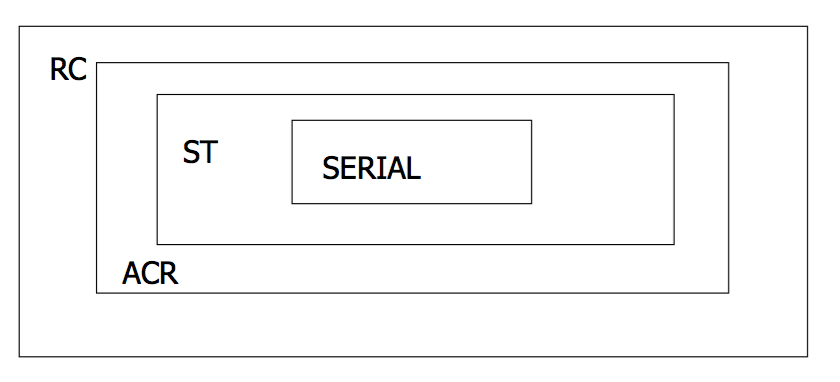
\includegraphics[scale=0.8]{img/FRCCDiagram}}
\caption{Venn Diagram}
\label{fig:FRCCDiagram}
\end{figure}
Connection with 2PL:
\begin{figure}[H]
\centering
\subfloat{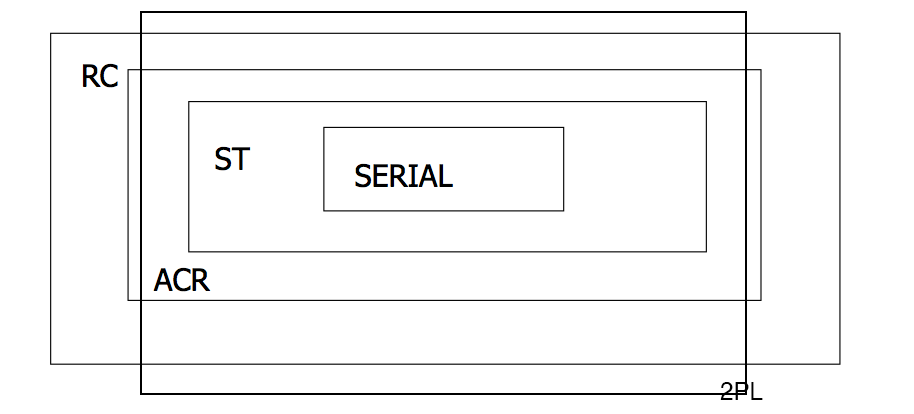
\includegraphics[scale=0.8]{img/FRCCDiagram2}}
\caption{Venn Diagram with 2PL}
\label{fig:FRCCDiagram}
\end{figure}
By convention serial $\ra$ 2PL

Strict 2PL: $\forall X, c_i <_S u_i(X)$. 

\begin{align*}
\text{serial} \ra \text{strict 2PL} \ra \text{strict} &\ra \text{2PL} \xrightarrow{\text{well-formed \& legal}}\text{conflict serializable}\\
&\ra \text{ACR} 
\end{align*}
\chapter{IVM, Incremental View Maintenance}
\section{Views}
\begin{enumerate}
\item Virtual View
\item Materialized View
\end{enumerate}


\section{Joins}
$$
V = \mat{L} \underset{C}\bowtie \mat{R}
$$

, where $C$ is the common attribute. 
\begin{enumerate}
\item Mediator-based join
\begin{enumerate}
\item Process: Ship to mediator
\item Issues: large traffic 
\end{enumerate}
\item Parameterized join
\begin{enumerate}
\item Process:
\begin{pseudo}
left = eval $Q_{\mat{L}}$
foreach C.val in left
  eval $Q_{\mat{R}, param=C.val}$
\end{pseudo}
\item Issues: multiple times of query
\end{enumerate}
\item Data ship join
\begin{enumerate}
\item Process:
\begin{pseudo}
left = eval $Q_{\mat{L}}$
ship left to $\mat{R}$
return left $\bowtie \mat{R}$ at $\mat{R}$
\end{pseudo}
\item Issue: traffic 
\end{enumerate}
\item Semijoin reduction join 
\begin{enumerate}
\item Process:
\begin{pseudo}
ship all $C.val$ of $\mat{R}$ to $\mat{L}$
semijoin = $\mat{L} \ltimes \mat{R}$
ship semijoin to $\mat{R}$
return semijoin $\bowtie \mat{R}$ at $\mat{R}$
\end{pseudo}
\end{enumerate}
\end{enumerate}
\section{IVM}
\subsection{Capturing}
Capturing IVM as computation of $\Delta V^+, \Delta V^-$. 

\subsubsection{$V$ with $\gamma$ aggregation}
\begin{itemize}
\item Input: $\Delta R^+, \Delta R^-$
\item Output: delete $\Delta V^-$ from V; insert $\Delta V^+$ into V;
\end{itemize}

\begin{pseudo}
$RG_+$ = select G, sum(A) as S from $\Delta R^+$ group by G;
$RG_-$ = select G, sum(A) as S from $\Delta R^-$ group by G;
$RG_{net}$ = select choose($RG_+$.G, $RG_-$.G) as G, n0($RG_+$.S)-n0($RG_-$.S) as S
         from $RG_+ \fullouterjoin RG_-$ on $RG_+$.C=$RG_-$.C;
$\Delta V^-$ = select * from V where G in (select G from $RG_{net}$);
$\Delta V^+$ = select $RG_{net}$.G as G, n0(V.S)+$RG_{net}$.S as S
        from V $\rightouterjoin RG_{net}$ on V.G=$RG_{net}$.G;
\end{pseudo}

, where choose(a,b) $\triangleq$ return a? a: b; n0(a) $\triangleq$ a? a: 0. These function definitions depend on the $\gamma$ function.

Modification on $\Delta V^+$: a possible fix is that the query computing the $\Delta V^+$ should include an EXISTS that checks whether the G value actually still appears in the table R.

\subsection{Methods}
\begin{enumerate}
\item Eager $\Delta R_i^+, \Delta R_i^-, R_i^0$
\item Deferred $\Delta R_i^+, \Delta R_i^-, R_i^1$
\item Self-maintained $\Delta R_i^+, \Delta R_i^-$
\end{enumerate}

\subsection{Algorithm for composing operators}
deferred version: $R$ means $R^1$, $S$ means $S^1$
\begin{itemize}
\item Rule for $V = R \bowtie S$
\begin{align*}
\Delta V^+ &= (\Delta R^+ \bowtie S) \cup (R \bowtie \Delta S^+) - (\Delta R^+ \bowtie \Delat \Delta S^+)\\
\Delta V^- &= (\Delta R^- \bowtie S) \cup (R \bowtie \Delta S^-) \cup (\Delta R^- \bowtie \Delat \Delta S^-)
\end{align*}
\item Rule for $V = \sigma_c R$
\begin{align*}
\Delta V^+ &= \sigma_c \Delta R^+\\
\Delta V^- &= \sigma_c \Delta R^-
\end{align*}
\item Compositions of rules $V = T\bowtie \sigma_c W$: $\Delta V^+, \Delta V^-$ simple composition of above rules 
\end{itemize}
eager version: $R$ means $R^0$, $S$ means $S^0$. Can derive eager version from deferred version:
\begin{align*}
\Delta V^+ &= (\Delta R^+ \bowtie S) \cup (R \bowtie \Delta S^+) \cup (\Delta R^+ \bowtie
\Delat \Delta S^+)\\
\Delta V^- &= (\Delta R^- \bowtie S) \cup (R \bowtie \Delta S^-) - (\Delta R^- \bowtie
\Delat \Delta S^-)
\end{align*}
\subsection{Caching}
\begin{align*}
\Pi_{G, H, G\#H\ra N, S}\ \gamma_{G, H; \text{SUM}(A) \ra S} R
\end{align*}

The problem, view $V_0$ in $f^+$ is not output of aggregation $\gamma$, but the output of projection $\Pi$. 

\textbf{Cache intermediate view on subexpression}. The solution, create an intermediate view on $\gamma$, i.e. the cache of intermediate result.

\textbf{Bottom up}. From updating caches to reaching the materialized view


\end{document}
